\chapter{Foundation}

\section*{Introduction}
This chapter details the implementation phase of our project, which follows an agile methodology with four sprints. Each sprint focuses on delivering specific features and functionality according to the project backlog. The implementation utilizes a modern tech stack consisting of React \cite{ReactWebsite} with Vite \cite{ViteJSWebsite} for the frontend, Node.js \cite{NodeJSWebsite} with Express.js \cite{ExpressJSWebsite} for the backend, MySQL \cite{MySQLWebsite} for database management, and Tailwind CSS \cite{TailwindWebsite} for styling.

Our first sprint focused on establishing essential foundational components of the system, with the following key deliverables:

\subsection{Web Backoffice Authentication}
\begin{itemize}
    \item Admin dashboard login and authentication system
    \item Role-based access control for backoffice users (Super Admin, Admin, Agent)
    \item User management interface for creating and managing user accounts
    \item Permission management system for different user roles
    \item Security logs and audit trails for backoffice activities
    \item Session management and secure token handling
\end{itemize}

\section{Sprint 1: Authentication and User Management }
\subsection*{Overview}
The first sprint focuses on establishing the core authentication system and user management functionality. This foundation is critical for all subsequent features as it defines user roles and access controls.


\subsection{Authentication and User Management System}
The Authentication and User Management system forms the backbone of Korpor's security and user interaction model. It encompasses processes for user registration with role assignment, secure login with session and token management, password recovery mechanisms, and session termination. Figure \ref{fig:auth-usermgmt-usecase} illustrates the global use cases for these core functionalities.

\begin{figure}[htbp]
    \centering
    % Replace with actual image file path
    % 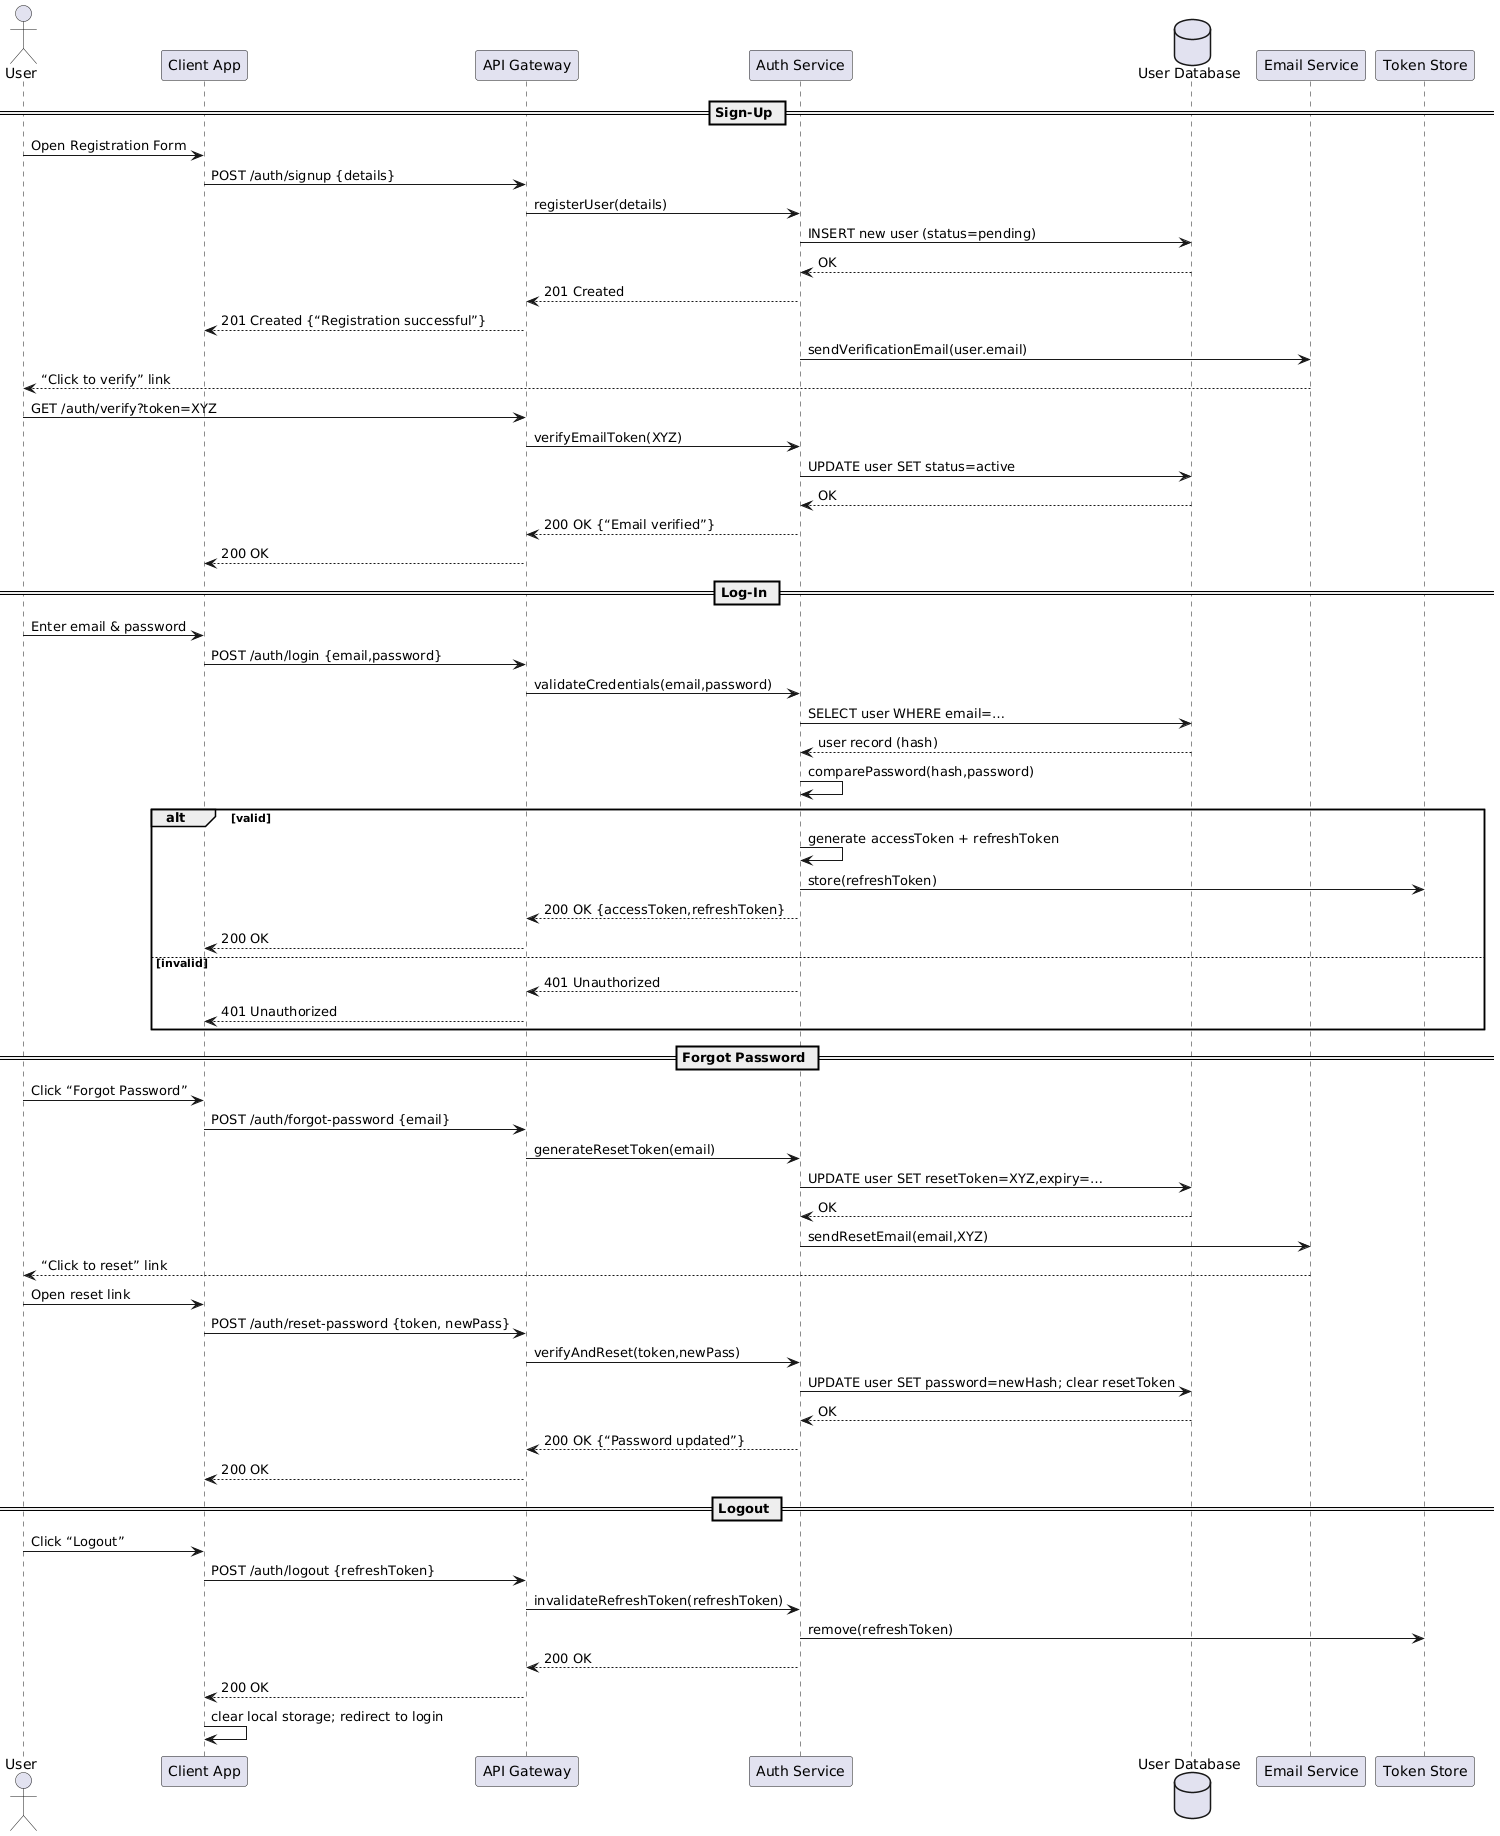
\includegraphics[width=0.9\textwidth]{images/auth-usermgmt-usecase.png} 
    \caption{Global Use Case Diagram for Authentication and User Management}
    \label{fig:auth-usermgmt-usecase}
\end{figure}
\newpage


\subsubsection{Sign-up Process}
The sign-up process is illustrated in Figure \ref{fig:signup-diagram} below. The diagram shows the authentication flow for new users registering in the system.

\begin{figure}[ht!]
    \centering
    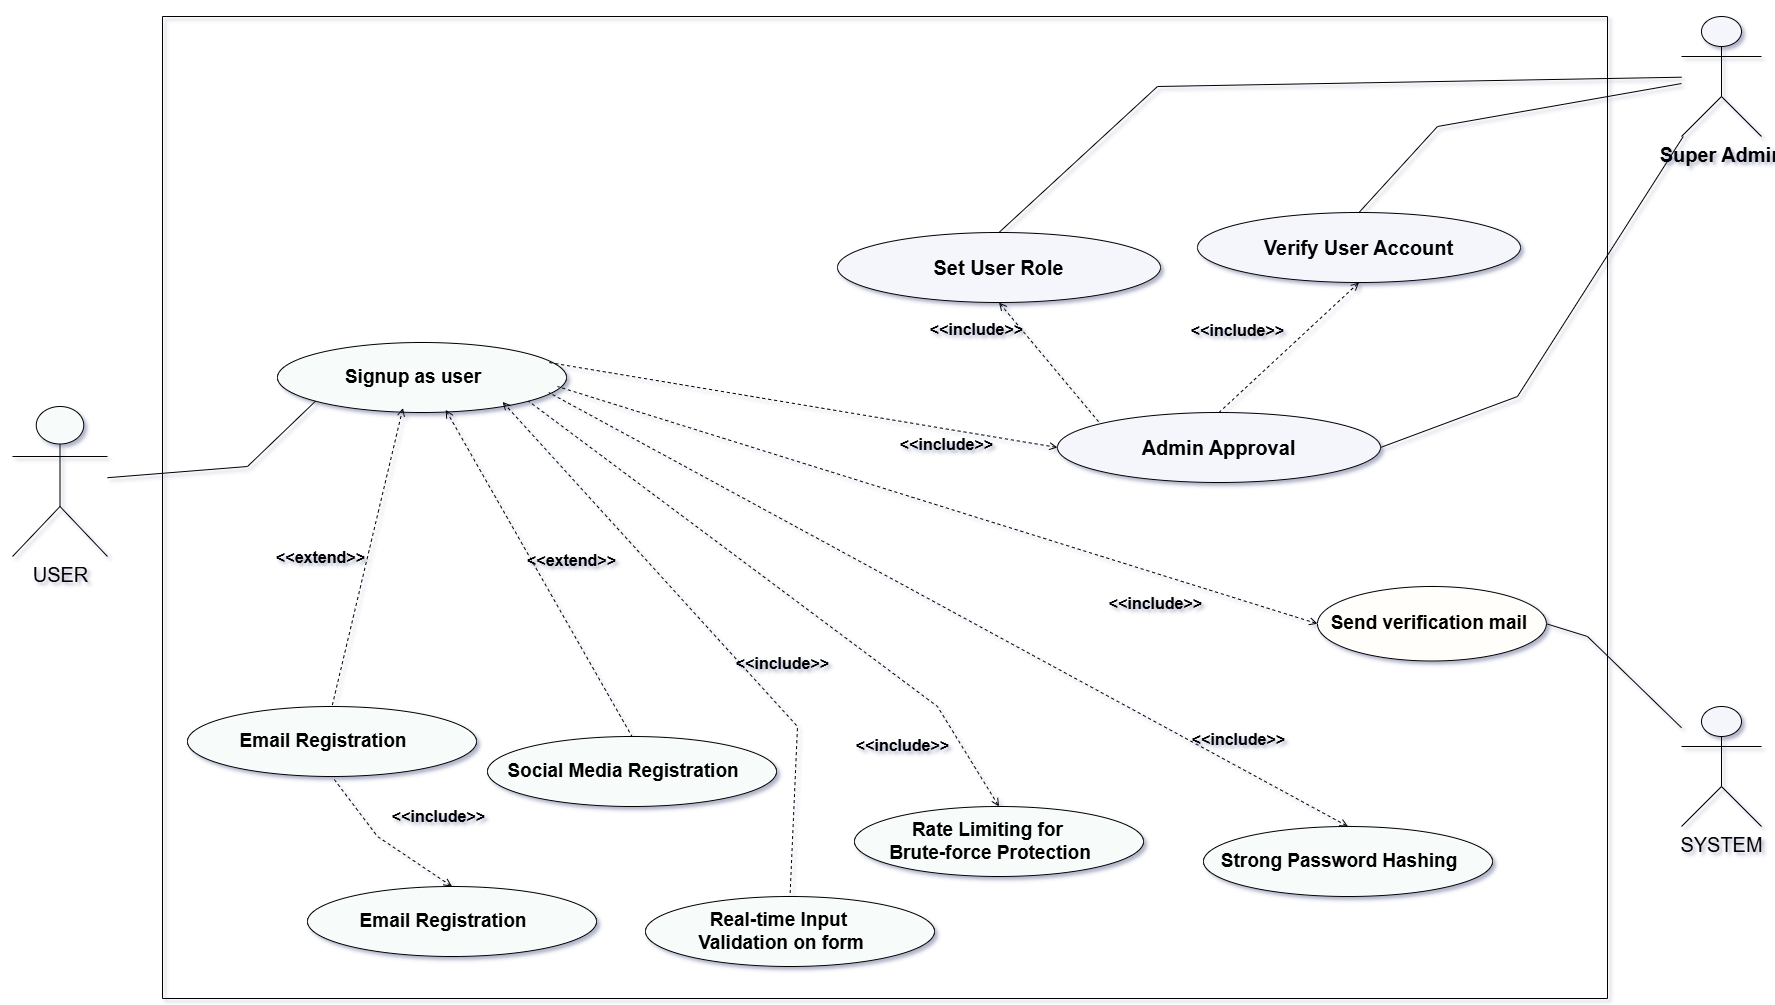
\includegraphics[width=1.03\textwidth]{images/diagram_de_case_d_utilisation_signup.png}
    \caption{Authentication Sign-up Use Case Diagram}
    \label{fig:signup-diagram}
\end{figure}

Figure \ref{fig:signup-activity-diagram} illustrates the activity flow of the sign-up process. The process begins when a new user navigates to the sign-up page and presses the sign-up button. The system then presents a form for the user to fill out. Upon submission, the system validates the entered information. 

If the information is invalid, the user is prompted to correct the form. If the information is valid, the system saves the user's details in the database and sends a verification email to the user. The user must then check their email. 

Upon successful email verification, the system redirects the user to an "email verification code" page or a similar confirmation step. The Super Admin is then involved in a two-step verification process. If the Super Admin accepts the user, their login is enabled. If the Super Admin refuses the user, the user's account is deleted. If the initial email verification step fails (e.g., there's an issue with the verification code), an error message is displayed to the user.

\newpage

\begin{figure}[ht!]
    \centering
    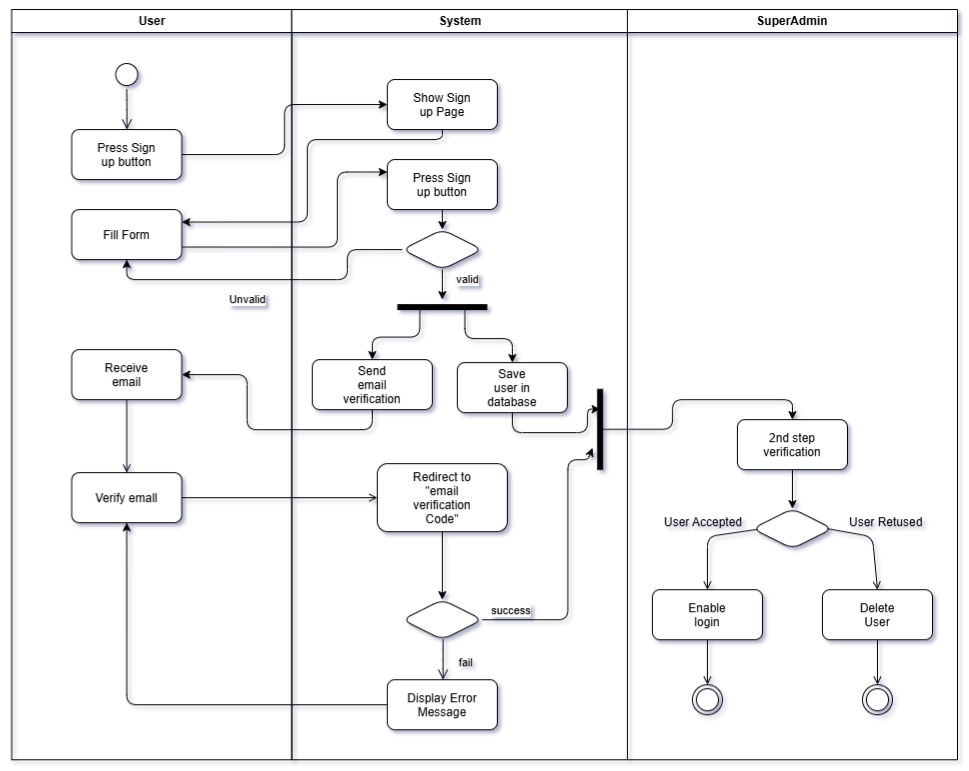
\includegraphics[width=1\textwidth]{images/signup_activitydiag.png}
    \caption{Authentication Sign-up Activity Diagram}
    \label{fig:signup-activity-diagram}
\end{figure}


% \vspace{1cm}

\subsubsection{Login Process}
The login process allows existing users to access the system. The table below details the use case.

\begin{table}[htbp]
    \centering
    \begin{tabular}{|l|p{0.7\textwidth}|}
        \hline
        \textbf{Section} & \textbf{Details} \\
        \hline
        Use Case & User Login \\
        \hline
        Actor & User (Super Admin, Admin, Agent, Investor) \\
        \hline
        Precondition & User has an existing, verified account. User is on the login page. \\
        \hline
        Main Scenario & 
        1. User enters their credentials (e.g., email and password).
        2. User clicks the login button.
        3. System verifies the credentials.
        4. If credentials are valid, the system grants access and redirects the user to their respective dashboard. \\
        \hline
        Postcondition & User is successfully logged into the system and can access features based on their role. \\
        \hline
        Exception & 
        - Invalid credentials: System displays an error message.
        - Account locked/disabled: System displays an appropriate message.
        - System error: System displays a general error message. \\
        \hline
    \end{tabular}
    \caption{Login Process Details}
    \label{tab:login_process}
\end{table}

\newpage
\subsubsection{Manage Users Process}
The user management process enables administrators to create, view, update, and delete user accounts. The table below details the use case.

\begin{table}[htbp]
    \centering
    \begin{tabular}{|l|p{0.7\textwidth}|}
        \hline
        \textbf{Section} & \textbf{Details} \\
        \hline
        Use Case & Assign Role \\
        \hline
        Actor & Super Admin \\
        \hline
        Precondition & Actor is logged into the system with appropriate administrative privileges. \\
        \hline
        Main Scenario & 
        1. Actor navigates to the user management section.
        2. To create a user: Actor fills in user details (name, email, role, etc.) and submits the form. System creates the new user account.
        3. To view users: System displays a list of users. Actor can search/filter the list.
        4. To update a user: Actor selects a user, modifies their details, and saves the changes. System updates the user account.
        5. To delete a user: Actor selects a user and confirms deletion. System deactivates or deletes the user account. \\
        \hline
        Postcondition & User account is created, updated, or deleted as per the action taken. The list of users reflects the changes. \\
        \hline
        Exception & 
        - Invalid input data: System displays validation errors.
        - Permission denied: System prevents unauthorized actions.
        - User not found (for update/delete): System displays an error message.
        - System error: System displays a general error message. \\
        \hline
    \end{tabular}
    \caption{Manage Users Process Details}
    \label{tab:manage_users_process}
\end{table}


The sign-up process includes user registration, role assignment, and account verification steps. During registration, users are categorized into one of the three user types: Super Admin, Admin, or Agent, with each type having different permissions and access levels within the system.

\newpage    

\begin{figure}[htbp]
    \centering
    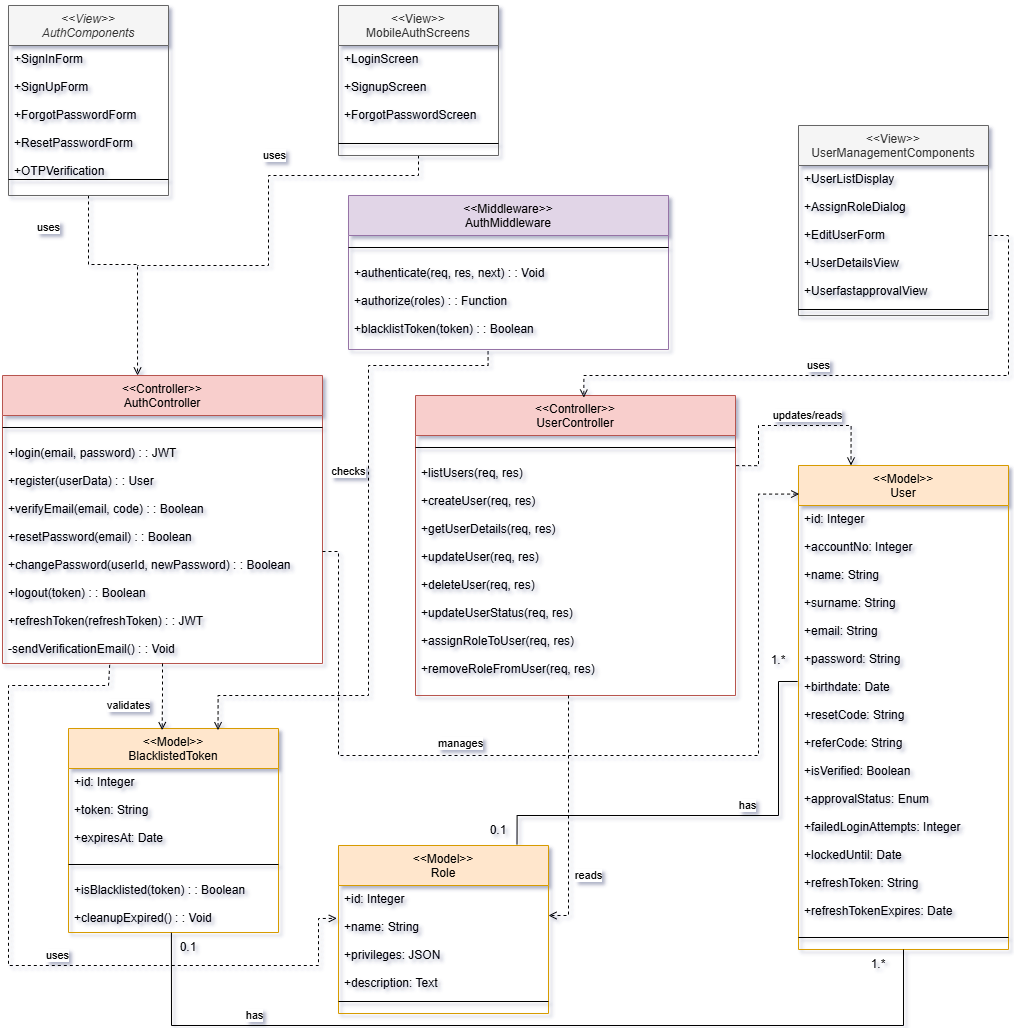
\includegraphics[width=1\textwidth]{images/auth_classdiag.PNG}
    \caption{Authentication AND User Management System Class Diagram}
    \label{fig:auth-class-diagram}
\end{figure}

Figure \ref{fig:auth-class-diagram} depicts the class diagram for the authentication system. It showcases the key components and their relationships involved in user authentication and authorization.

\newpage

\begin{itemize}
    \item \textbf{AuthComponents}: Represents the UI elements for authentication, such as SignInForm, SignUpForm, ForgotPasswordForm, ResetPasswordForm, and OTPVerification. These components are used by \textbf{MobileAuthScreens}.
    \item \textbf{MobileAuthScreens}: Includes screens like LoginScreen, SignupScreen, and ForgotPasswordScreen that utilize \textbf{AuthComponents} and interact with the \textbf{AuthService}.
    \item \textbf{AuthService}: Acts as an intermediary between the frontend components/screens and the backend. It handles functions like signIn, signUp, verifyEmail, forgotPassword, resetPassword, logout, refreshToken, and error handling. It consumes \textbf{AuthRoutes}.
    \item \textbf{AuthRoutes}: Defines the API endpoints for authentication, such as /login, /register, /verify-email, /forgot-password, /reset-password, /logout, and /refresh-token. These routes map to methods in the \textbf{AuthController}.
    \item \textbf{AuthController}: Contains the core logic for authentication processes, including login, register, verifyEmail, resetPassword, changePassword, logout, refreshToken, and sendVerificationEmail. It interacts with the \textbf{User}, \textbf{Role}, and \textbf{BlacklistedToken} models and utilizes \textbf{AuthMiddleware}.
    \item \textbf{AuthMiddleware}: Provides middleware functions for authentication (authenticate) and authorization (authorize roles). It also manages blacklisted tokens (blacklistToken) and interacts with the \textbf{User} model.
    \item \textbf{User}: Represents the user entity with attributes like id, accountNo, name, surname, email, password, birthdate, resetCode, isVerified, approvalStatus, failedLoginAttempts, lockedUntil, refreshToken, and refreshTokenExpires. A User has one or more \textbf{Role}s.
    \item \textbf{Role}: Defines user roles with attributes like id, name, privileges (JSON), and description. Each User is associated with a Role (0..1 relationship shown, typically a User has at least one Role, but the diagram indicates a User can have zero or one Role, which might need clarification or represent a specific system design choice, e.g., a default role or a user awaiting role assignment).
    \item \textbf{BlacklistedToken}: Stores tokens that have been invalidated (e.g., after logout or password change) with attributes like id, token, and expiresAt. It includes methods like isBlacklisted and cleanupExpired. The \textbf{AuthController} uses this to validate tokens, and \textbf{AuthMiddleware} checks against it.
\end{itemize}

\subsection{Implementation Interfaces}
The implementation of the authentication and user management system resulted in the following key user interfaces:

\subsubsection{Sign-in Interface}
The sign-in interface provides a secure and user-friendly means for users to authenticate. Figure \ref{fig:signin-interface} shows the implementation of this interface.
\newpage
\begin{figure}[htbp]
    \centering
    % Add correct path when available
    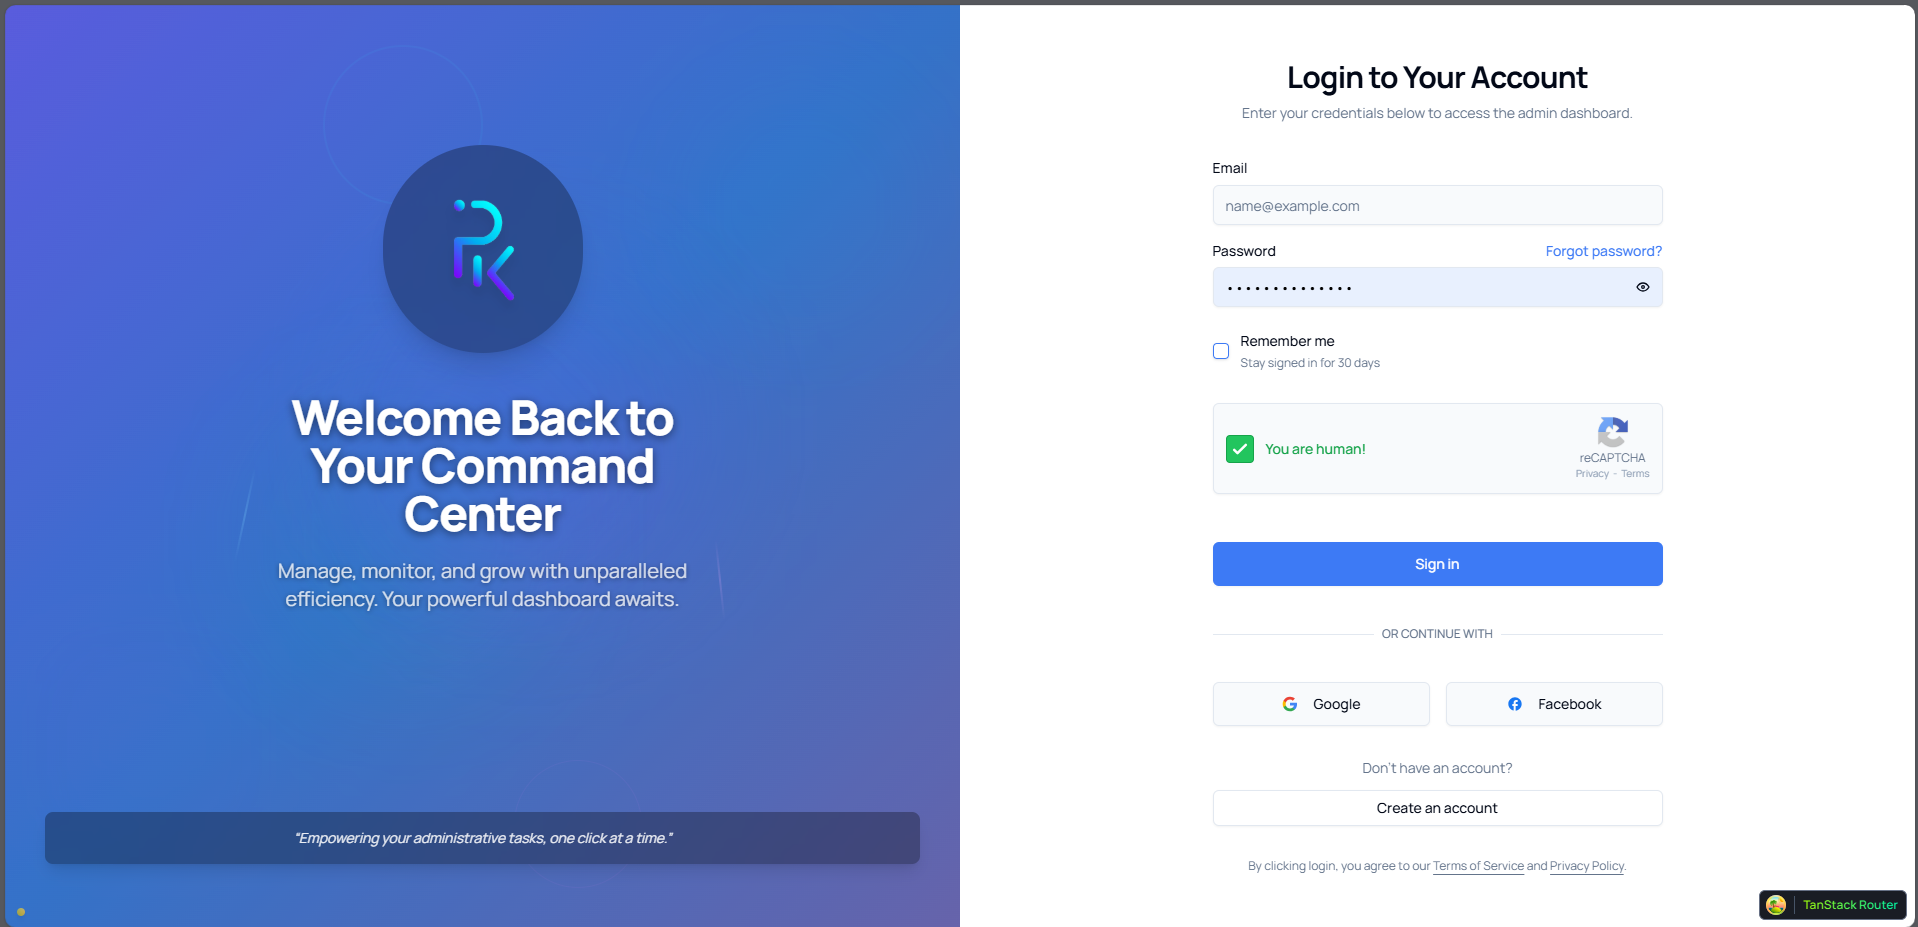
\includegraphics[width=1\textwidth]{images/signin-interface.png}
    \caption{Sign-in Interface Implementation}
    \label{fig:signin-interface}
\end{figure}

\subsubsection{Sign-up Interface}
The sign-up interface allows new users to register for an account. It collects necessary information and begins the verification process. Figure \ref{fig:signup-interface} displays this implementation.

\begin{figure}[htbp]
    \centering
    % Add correct path when available
    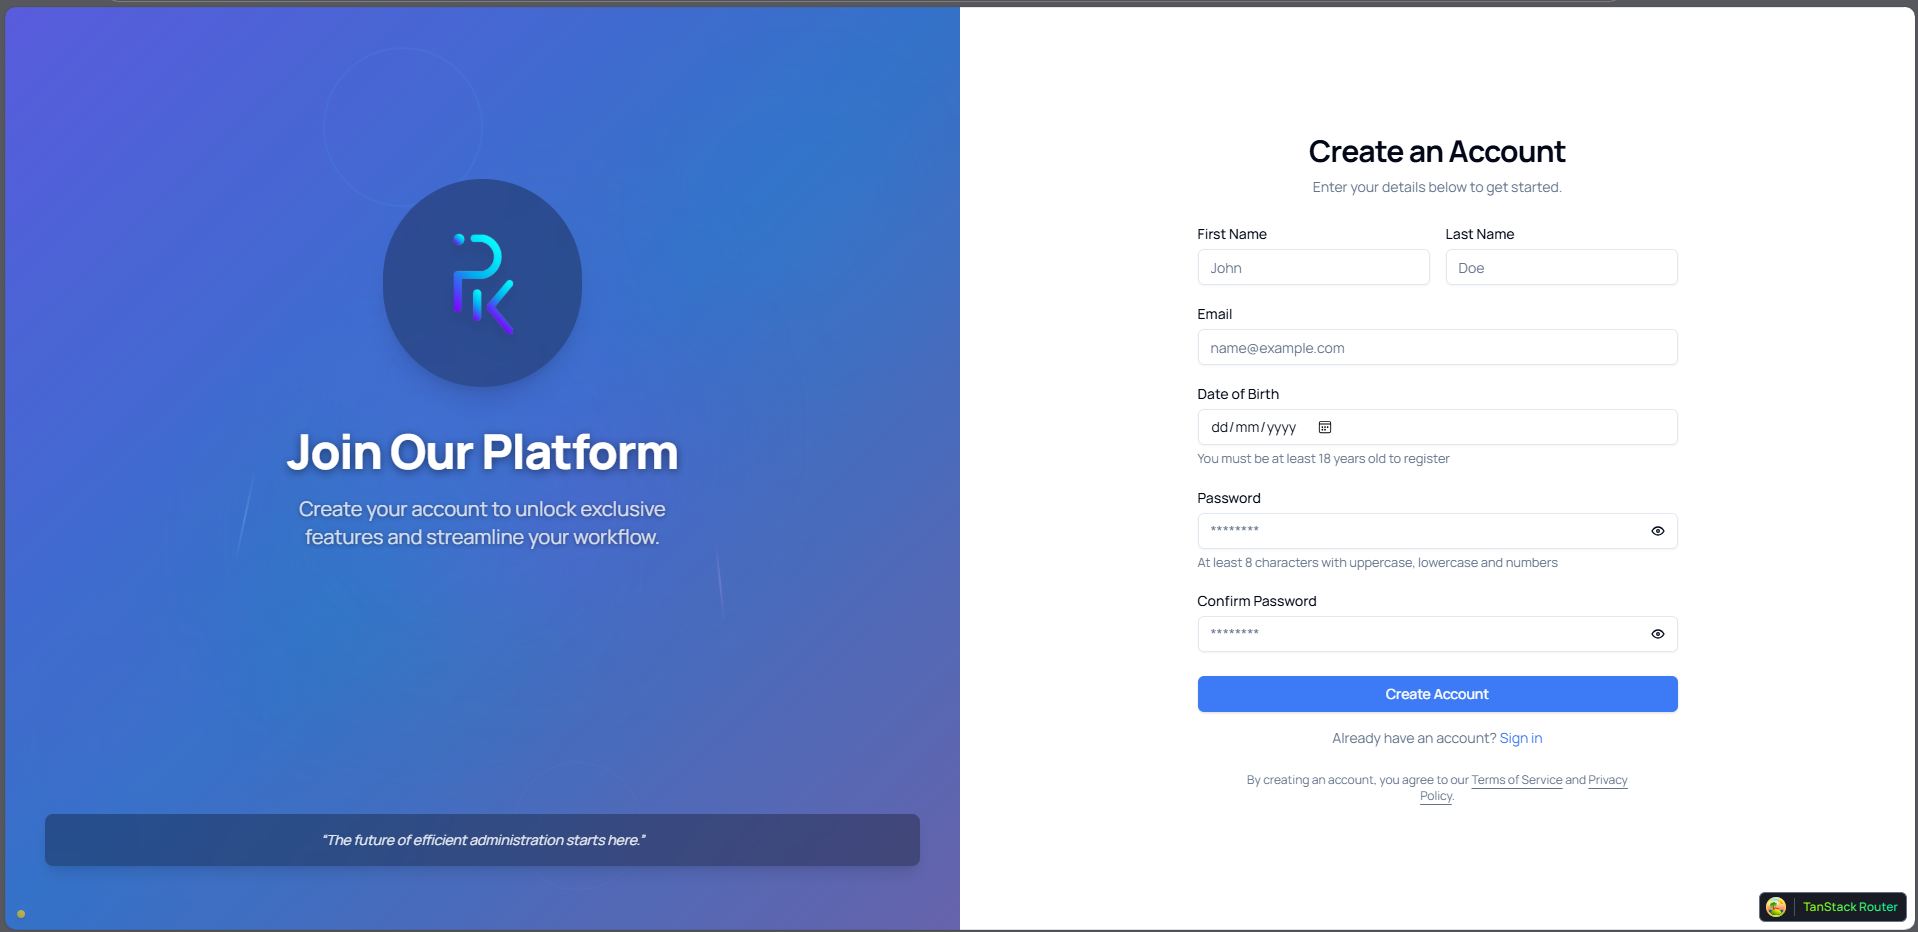
\includegraphics[width=1\textwidth]{images/signup-interface.png}
    \caption{Sign-up Interface Implementation}
    \label{fig:signup-interface}
\end{figure}

\subsubsection{User Management in Super Admin Dashboard}
The Super Admin dashboard provides comprehensive user management capabilities, including the ability to view, create, edit, and deactivate user accounts. Figure \ref{fig:user-management} shows this powerful interface.
\newpage
\begin{figure}[htbp]
    \centering
    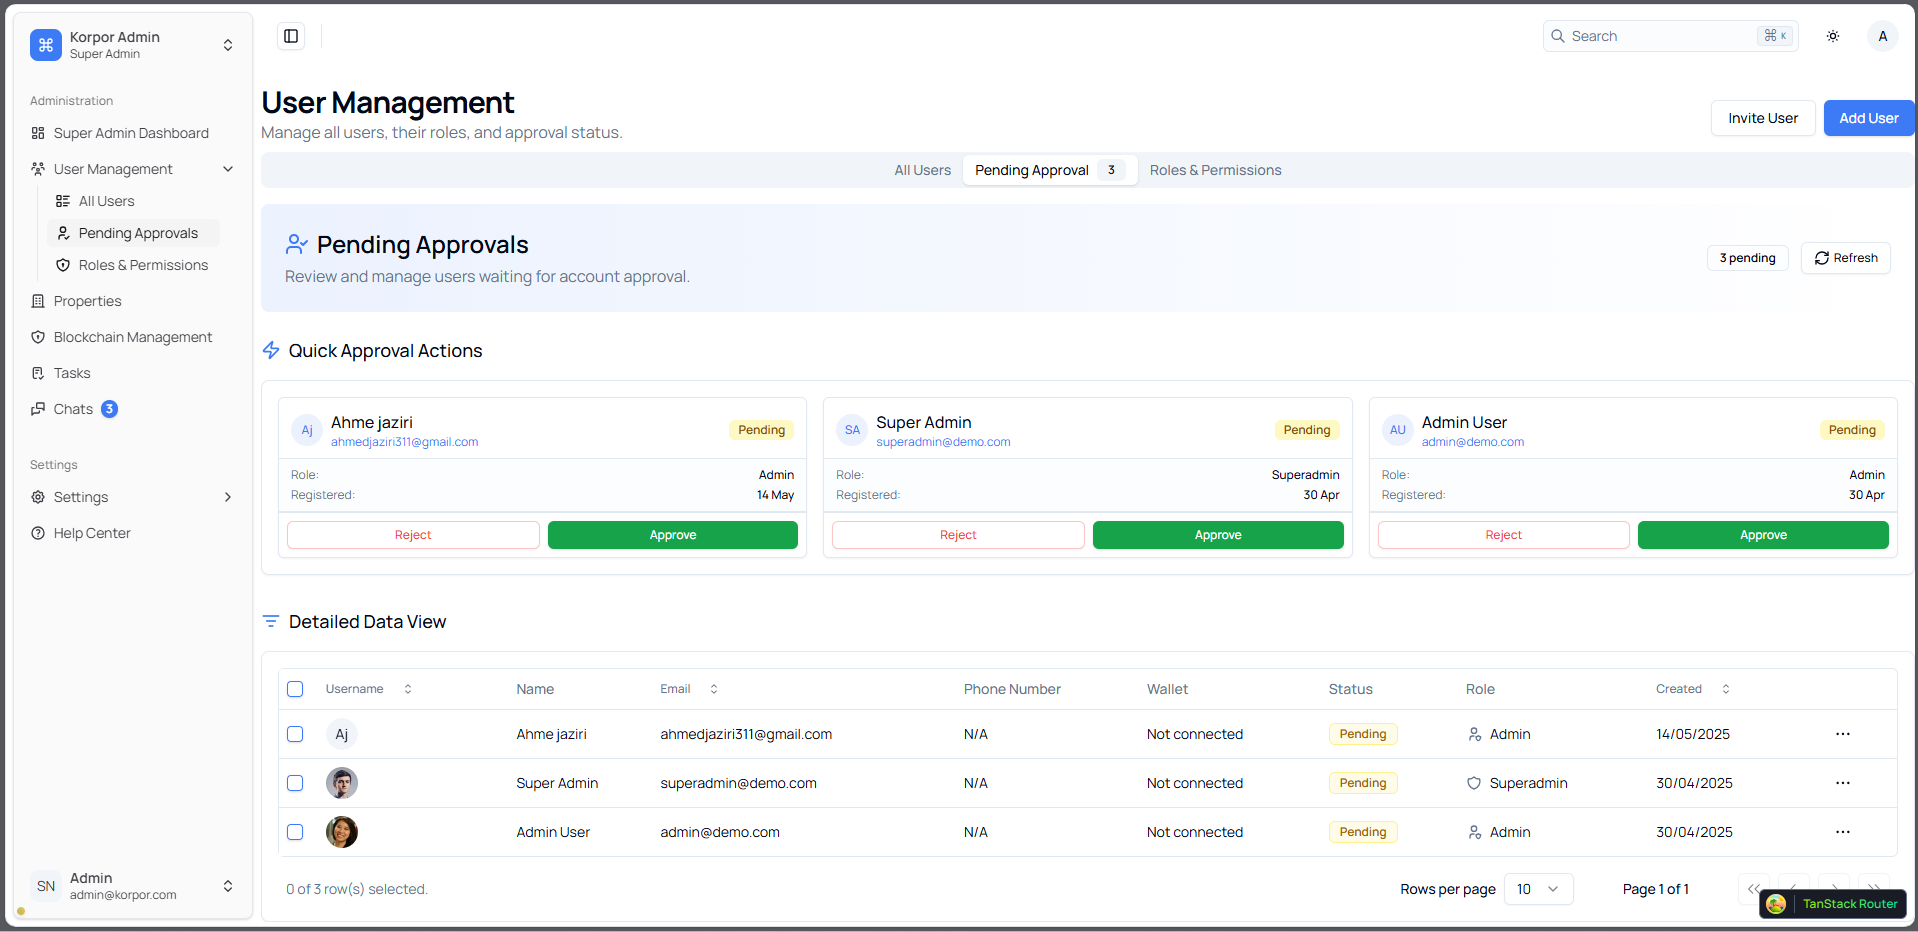
\includegraphics[width=1\textwidth]{images/user-management-dashboard.png}
    \caption{User Management Interface in Super Admin Dashboard}
    \label{fig:user-management}
\end{figure}

\subsection{Mobile Application Interfaces}
The mobile application provides a streamlined authentication experience for investors. The system includes comprehensive error handling to guide users through common authentication issues, as shown in Figure \ref{fig:mobile-auth-errors}. The complete authentication flow includes login, signup, OTP verification, and password recovery interfaces designed for clarity and ease of use on mobile devices, as shown in Figure \ref{fig:mobile-auth-interfaces}.
\begin{figure}[htbp]
    \centering
    \begin{subfigure}[b]{0.45\textwidth}
        \centering
        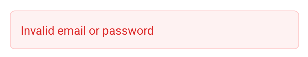
\includegraphics[width=\textwidth]{images/mobile-auth-screen_invalidemailorpass.png}
        \caption{Invalid Email or Password Error}
        \label{fig:mobile-invalid-credentials}
    \end{subfigure}
    \hfill
    \begin{subfigure}[b]{0.45\textwidth}
        \centering
        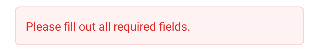
\includegraphics[width=\textwidth]{images/mobile-auth-screen_emptyfieldsmessage.png}
        \caption{Empty Fields Validation Error}
        \label{fig:mobile-empty-fields}
    \end{subfigure}
    \caption{Authentication Validation Messages}
    \label{fig:mobile-auth-errors}
\end{figure}
% \subsubsection{Complete invastor Authentication Flow}


\begin{figure}[htbp]
    \centering
    % First row - 3 screens
    \begin{subfigure}[b]{0.3\textwidth}
        \centering
        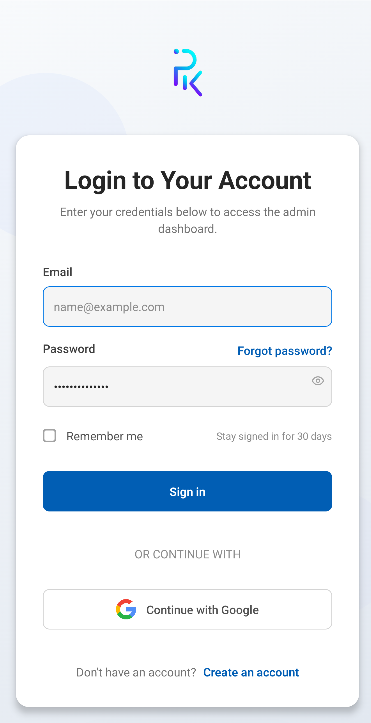
\includegraphics[width=\textwidth]{images/mobile-auth-screen_login.png}
        \caption{Login Screen}
        \label{fig:mobile-login}
    \end{subfigure}
    \hfill
    \begin{subfigure}[b]{0.3\textwidth}
        \centering
        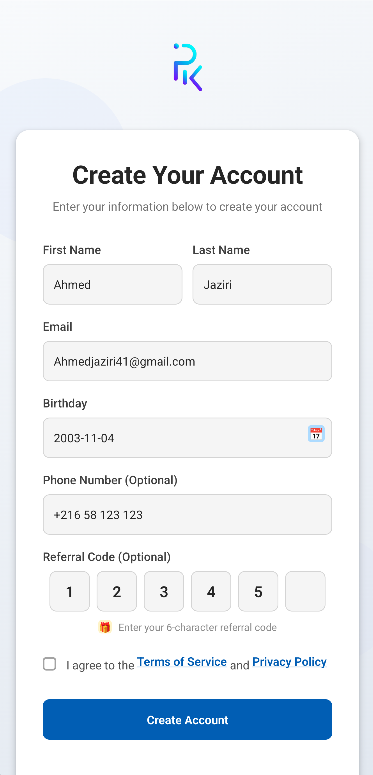
\includegraphics[width=\textwidth]{images/mobile-auth-screen_signup.png}
        \caption{Signup Screen}
        \label{fig:mobile-signup}
    \end{subfigure}
    \hfill
    \begin{subfigure}[b]{0.3\textwidth}
        \centering
        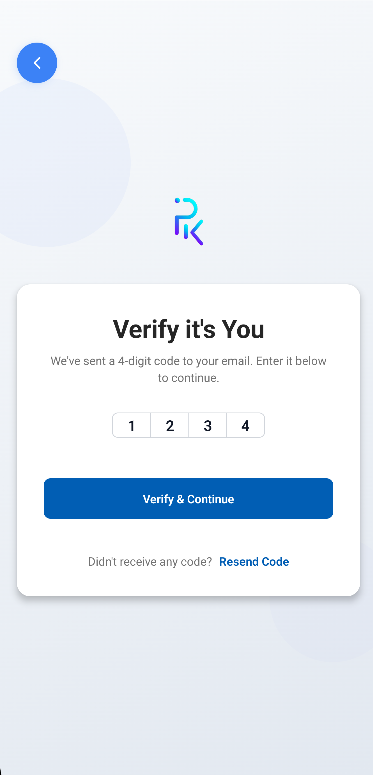
\includegraphics[width=\textwidth]{images/mobile-auth-screen_otp.png}
        \caption{OTP Verification Screen}
        \label{fig:mobile-otp}
    \end{subfigure}
    
    \vspace{0.5cm} % Add some vertical space between rows
    
    % Second row - 2 screens (centered)
    \begin{subfigure}[b]{0.3\textwidth}
        \centering
        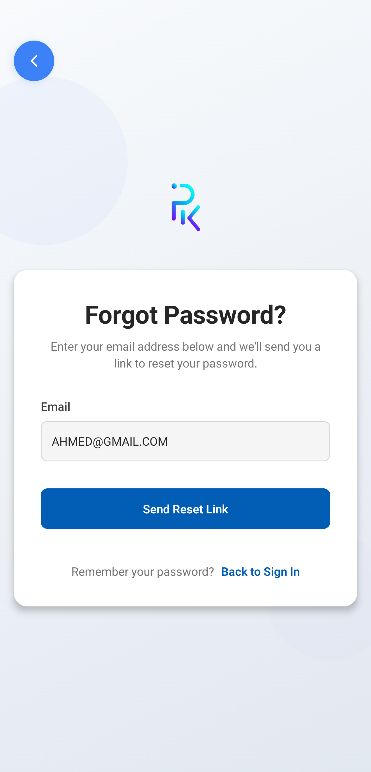
\includegraphics[width=\textwidth]{images/mobile-auth-screen_forgetpassword.png}
        \caption{Forgot Password Screen}
        \label{fig:mobile-forgot-password}
    \end{subfigure}
    \hfill
    \begin{subfigure}[b]{0.3\textwidth}
        \centering
        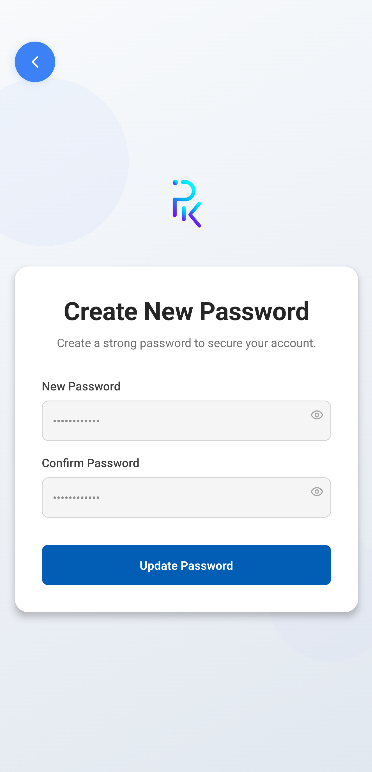
\includegraphics[width=\textwidth]{images/mobile-auth-screen_newpassword.png}
        \caption{New Password Screen}
        \label{fig:mobile-new-password}
    \end{subfigure}
    \caption{Complete Mobile Application Authentication Flow}
    \label{fig:mobile-auth-interfaces}
\end{figure}

\newpage

\subsection{Testing Validation}
To ensure the reliability and functionality of the authentication and user management system, we implemented comprehensive testing using Playwright, an end-to-end testing framework \cite{PlaywrightDocs2023}.

\subsubsection{Playwright Test Results}
The authentication system underwent rigorous testing through automated test scripts that verified all key functionality, including sign-up, sign-in, password reset, and user management operations. Figure \ref{fig:playwright-tests} demonstrates the successful execution of these tests.
\begin{figure}[htbp]
    \centering
    % Add correct path when available
    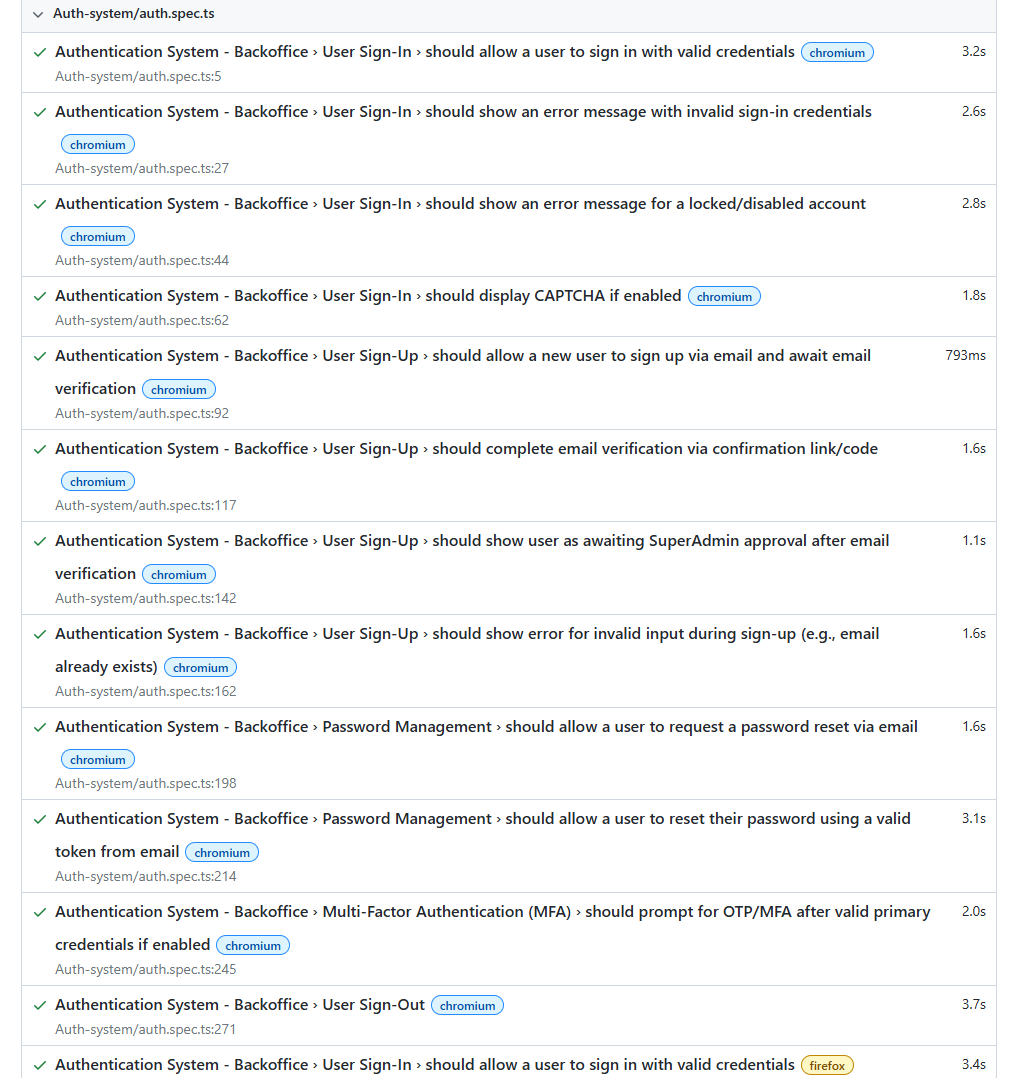
\includegraphics[width=0.65\textwidth]{images/playwright-test-results.png}
    \caption{Playwright Test Results for Authentication System}
    \label{fig:playwright-tests}
\end{figure}


All tests passed successfully, confirming the robustness of the implemented authentication system.

\section*{Conclusion}

The Foundation sprint successfully established the secure authentication and user management infrastructure for the Korpor platform.

% Additional sections for subsequent sprints will be added later 